\documentclass[11pt]{article}
\usepackage[T1]{fontenc}
\usepackage{lmodern}
\usepackage[margin=1in]{geometry}
\usepackage{amsmath,amssymb,amsthm}
\usepackage{microtype}
\usepackage{flafter}
\usepackage{enumitem}
\usepackage{tikz}
\usetikzlibrary{arrows.meta,positioning}
\usepackage[colorlinks=true,linkcolor=blue!45!black,citecolor=blue!45!black,urlcolor=blue!45!black]{hyperref}
\hypersetup{pdftitle={A superquadratic separation between sensitivity and block sensitivity},pdfauthor={OpenAI}}
\newcommand{\bs}{\operatorname{bs}}
\newcommand{\unverified}[1]{\par\smallskip\noindent\fbox{\parbox{0.95\linewidth}{\textbf{Unverified step.} #1}}\par\smallskip}
\newtheorem{theorem}{Theorem}[section]
\newtheorem{lemma}[theorem]{Lemma}
\newtheorem{proposition}[theorem]{Proposition}
\newtheorem{corollary}[theorem]{Corollary}
\theoremstyle{definition}
\newtheorem{definition}[theorem]{Definition}
\theoremstyle{remark}
\newtheorem{remark}[theorem]{Remark}
\title{A superquadratic separation between sensitivity\\and block sensitivity}
\author{Rewritten for readability from the OpenAI manuscript of the same title}
\date{September 25, 2026}
\begin{document}
\maketitle
\begin{abstract}
We disprove the quadratic strengthening of the Sensitivity Conjecture by
constructing nonconstant total Boolean functions whose block sensitivity grows
faster than any constant multiple of sensitivity squared. In fact, for some
fixed \(\alpha>2\), composed examples (Corollary~\ref{cor:power-separation})
have unbounded block sensitivity and satisfy \(\bs(f)\ge s(f)^\alpha\).
\end{abstract}

\section{Introduction}
\label{sec:introduction}

\paragraph{Definitions.}
For a positive integer $n$ write $[n]=\{1,\ldots,n\}$. For $x\in\{0,1\}^n$ and
$B\subseteq[n]$, let $x^B$ be $x$ with exactly the coordinates in $B$ flipped,
and write $x^e=x^{\{e\}}$. (The source writes $x^a$; we call a single
coordinate $e$ because $a(i,j)$ will denote edge labels.) In particular $0^B$
is the indicator string of $B$. For a total Boolean function
$f:\{0,1\}^n\to\{0,1\}$,
\[
 s(f,x)=\bigl|\{e\in[n]:f(x^e)\ne f(x)\}\bigr|,\qquad s(f)=\max_x s(f,x).
\]
A nonempty $B\subseteq[n]$ with $f(x^B)\ne f(x)$ is a \emph{sensitive block}
of $f$ at $x$. The block sensitivity $\bs(f,x)$ is the largest number of
pairwise disjoint sensitive blocks at $x$, and $\bs(f)=\max_x\bs(f,x)$.

\begin{theorem}\label{thm:main}
For every real \(C>0\), there are a positive integer \(n\) and a
nonconstant total Boolean function \(f:\{0,1\}^n\to\{0,1\}\) such that
\[
 \bs(f)>C\,s(f)^2.
\]
More precisely, for every integer \(d\ge1\) the construction below gives
a nonconstant total Boolean function \(f\) with
\[
 \frac{\bs(f)}{s(f)^2}\ge \frac{2^d}{4(d+2)^2}.
\]
\end{theorem}

Section~\ref{sec:separation} also proves
Corollary~\ref{cor:power-separation}: a fixed $\alpha>2$ and functions $F_m$
with $\bs(F_m,0)\ge s(F_m)^\alpha$ and $\bs(F_m,0)\to\infty$. Since
$\bs(F_m)\ge\bs(F_m,0)$, this is the second claim of the abstract.

\paragraph{Background.}
The Sensitivity Conjecture asked whether block sensitivity is bounded by a
polynomial in sensitivity. It goes back to Nisan, who introduced block
sensitivity and recorded Rubinstein's quadratic separation
\cite[Section~2]{Nisan1989}; Nisan and Szegedy suggested
$\bs(f)\le s(f)^2$ \cite[Section~4]{NisanSzegedy1994}. Rubinstein's
construction \cite{Rubinstein1995} showed that a polynomial bound needs degree
at least two; Virza obtained $\bs(f)=\tfrac12s(f)^2+\tfrac12s(f)$
\cite{Virza2011} and Ambainis and Sun
$\bs(f)=\tfrac23s(f)^2-\tfrac13s(f)$ \cite[Theorem~1]{AmbainisSun2011}.
Huang's degree bound with Tal's refinement \cite{Tal2013} gives
$\bs(f)\le s(f)^4$ \cite[Theorem~1.5]{Huang2019}, improved by Wellens to
$\bs(f)\le\sqrt{2/3}\,s(f)^4+1$ \cite[Corollary~4.2]{Wellens2022}.
Theorem~\ref{thm:main} rules out every bound $\bs(f)\le Cs(f)^2$.

The architecture (tournament-indexed rows, one selected blocking coordinate in
each outgoing row, random labels) adapts Meiburg's spectral-sensitivity
construction \cite[Sections~3.1 and~5.2--5.5]{Meiburg2026}\footnote{In the
attribution accompanying this construction, Meiburg credits GPT-5.6-Sol
with the gated-tournament ideas and describes his own contributions as
exposition, size and parameter optimization, and checking the faithfulness
of the Lean formalization.}, here with nested predicates and a different
forbidden-label condition (Lemma~\ref{lem:labelling}). Spectral sensitivity
$\lambda(f)$ \cite{AaronsonEtAl2021} satisfies $\lambda(f)\le s(f)$, so a
lower bound on $\bs(f)/\lambda(f)^2$ does not give Theorem~\ref{thm:main};
the estimates below are proved directly. The final OR follows Ambainis and Sun
\cite[Section~4, Lemma~1]{AmbainisSun2011}. Ambainis and Pr\={u}sis noted that
a seed with $\bs>s^2$ yields a superquadratic power separation by iteration
\cite[Section~1]{AmbainisPrusis2014}; composition is treated systematically by
Tal~\cite{Tal2013}.

\paragraph{Proof at a glance.}
For levels $\ell=0,\ldots,d$ we build predicates
$P_{\ell,1}\ge P_{\ell,2}\ge\cdots$ (pointwise). A level-$\ell$ input is a
$k\times r$ array of level-$(\ell-1)$ inputs (``children''), with
$k=2M^2+1$ rows. Each $P_{\ell,q}$ is an OR of $k$ clauses, one per row.
Clause $i$ requires the strongest child predicate to accept every child of row
$i$ (\emph{targets}) and a weaker child predicate to reject one labelled child
in each of $M^2$ other rows (\emph{gates}); a tournament on the rows decides
which rows, and the index $q$ decides which weaker predicate. Each level
multiplies the number of disjoint sensitive blocks at $0$ by $k>2M^2$, but the
sensitivity by only about $M$; so $\bs/s^2$ gains a factor $>2$ per level.

\begin{enumerate}[leftmargin=*,itemsep=1pt]
\item Lemma~\ref{lem:labelling}: a labelling of tournament edges avoiding a
 certain 16-vertex pattern (union bound). Used only in step~C2 of
 Proposition~\ref{prop:recurrences}.
\item Lemma~\ref{lem:base}: sensitivity bounds at level $0$. Starts the
 induction in Lemma~\ref{lem:quantitative-profiles}.
\item Lemma~\ref{lem:blocks}: $Mk^\ell$ disjoint sensitive blocks at $0$ on
 level $\ell$. Used in the proof of Theorem~\ref{thm:main}.
\item Proposition~\ref{prop:recurrences} (the core): recurrences for
 $S_{\ell,b}$ (number of flips taking a predicate from $b$ to $1-b$) and
 $J_{\ell,b}$ (number of flips taking two predicates from $b$ to $1-b$
 simultaneously). The $J$'s are needed because repairing a failed gate usually
 forces \emph{two} child predicates to change, which is much rarer than one.
\item Lemma~\ref{lem:quantitative-profiles}: for $M\ge9^{d+1}$,
 $S_{\ell,b}\le2(d+2)M^{\ell+b}$ (from items 2 and 4).
\item Theorem~\ref{thm:main}: an OR of $M$ copies of $P_{d,1}$ balances
 $S_{d,0}$ against $S_{d,1}$ (from items 3 and 5).
\item Lemma~\ref{lem:composition} and
 Corollary~\ref{cor:power-separation}: composing the $d=9$ function with
 itself.
\end{enumerate}

\section{The labelled tournament and nested predicates}
\label{sec:construction}

Fix integers \(d\ge1\) and \(M\ge3\) ($M$ is chosen in terms of $d$ in
Section~\ref{sec:separation}), and put
\[
 L=d+2,\qquad k=2M^2+1,\qquad r=\lceil\sqrt M\rceil,\qquad t=16.
\]
A tournament orients every pair of distinct vertices: exactly one of
\(i\to j\), \(j\to i\) holds. Fix a tournament on \([k]\) in which every
vertex has outdegree \(M^2\); for example, place the $2M^2+1$ vertices on a
cycle and direct each vertex to the next \(M^2\) vertices.

\begin{lemma}\label{lem:labelling}
The edges can be labelled by numbers \(a(i,j)\in[r]\) so that there is
no set \(I\subseteq[k]\) of size \(t\) admitting choices
\(m_j\in[r]\), \(j\in I\), with
\[
 a(i,j)=m_j \qquad\text{for every edge }i\to j\text{ within }I.
\]
\end{lemma}
\begin{proof}
Choose all labels independently and uniformly from \([r]\). Fix \(I\) with
$|I|=16$ and \((m_j)_{j\in I}\). Every pair of vertices of $I$ carries exactly
one edge, so there are $\binom{16}{2}=120$ edges within $I$. The stated
equalities prescribe the labels of these 120 distinct edges, so they all hold
with probability \(r^{-120}\). There are at most
$\binom{k}{16}r^{16}\le k^{16}r^{16}$ choices of $(I,(m_j))$, so the
probability that some choice satisfies all its equalities is at most
\[
 k^{16}r^{16}r^{-120}=k^{16}r^{-104}\le (3M^2)^{16}(\sqrt M)^{-104}
 =3^{16}M^{32-52}=3^{16}M^{-20}\le3^{-4}<1,
\]
using \(k=2M^2+1\le3M^2\), \(r\ge\sqrt M\), and \(M\ge3\). Hence a suitable
labelling exists.
\end{proof}

Fix such a labelling. For \(0\le\ell\le d\) set
\[
 H_\ell=d+1-\ell,\qquad N_\ell=LM(kr)^\ell.
\]
We define predicates \(P_{\ell,q}:\{0,1\}^{N_\ell}\to\{0,1\}\),
\(1\le q\le H_\ell\), satisfying
\begin{description}[leftmargin=*,itemsep=1pt]
\item[\textup{(N)}] \emph{Nesting.}
 \(P_{\ell,1}(x)\ge P_{\ell,2}(x)\ge\cdots\ge P_{\ell,H_\ell}(x)\) for every
 \(x\).
\end{description}
Thus if $P_{\ell,q}(x)=0$ then every predicate of larger index is $0$ at
$x$, and if $P_{\ell,q}(x)=1$ then every predicate of smaller index is $1$ at
$x$. Nesting concerns the index $q$, not the input bits.

\subsection{Initial predicates}
Partition \([LM]\) into \(M\) blocks \(E_1,\ldots,E_M\) of size \(L\) and let
\(z_j=0^{E_j}\). With \(\operatorname{dist}\) the Hamming distance, set
\[
 D(x)=\min_{j\in[M]}\operatorname{dist}(x,z_j),\qquad
 P_{0,q}(x)=\mathbf1\{D(x)\le d+1-q\}\quad(1\le q\le d+1).
\]
So $P_{0,q}$ indicates the union of the Hamming balls of radius
$d+1-q\in\{0,\ldots,d\}$ around the centres $z_j$. (N) holds because the
radius decreases with $q$. Distinct centres are at distance \(2L=2d+4\).

\subsection{Recursive clauses}
Let \(1\le\ell\le d\). Put \(H=H_\ell\) and \(Q=H+1=H_{\ell-1}\), and
abbreviate
\[
 p_\gamma=P_{\ell-1,\gamma}\qquad(1\le\gamma\le Q)
\]
(our shorthand); by (N) at level $\ell-1$, $p_1\ge\cdots\ge p_Q$, so $p_Q$ is
the strongest. Split \(x\in\{0,1\}^{N_\ell}\) into \(kr\) disjoint children
\(x_{j,c}\in\{0,1\}^{N_{\ell-1}}\), with row \(j\in[k]\) and position
\(c\in[r]\); this uses $N_\ell=krN_{\ell-1}$. For $i\in[k]$ and \(q\in[H]\),
\emph{clause \(i\) at index \(q\)} asserts
\begin{equation}\label{eq:predicate-definition}
 \begin{aligned}
 p_Q(x_{i,c})&=1 &&\text{for all }c\in[r] &&\text{(\emph{target conditions})},\\
 p_{Q-q}(x_{j,a(i,j)})&=0 &&\text{for all }j\text{ with }i\to j &&\text{(\emph{gate conditions})}.
 \end{aligned}
\end{equation}
Define \(P_{\ell,q}(x)=1\) if clause $i$ at index $q$ holds for some $i$, and
$0$ otherwise. Indices are valid: \(1\le Q-q\le H<Q\). Two facts are used
throughout.
\begin{description}[leftmargin=*,itemsep=1pt]
\item[\textup{(DC)}] \emph{Distinct children.} For fixed $i$, the $r+M^2$
 conditions of clause $i$ sit on distinct children, the same ones for every
 $q$: targets occupy row $i$, and the gates lie in distinct rows $j\ne i$
 (there is one edge from $i$ to $j$). A single coordinate of $x$ lies in one
 child, so flipping it changes the truth value of at most one condition of
 clause $i$. (One child may occur in many clauses; we handle this by union
 bounds.)
\item[\textup{(Mon)}] \emph{Monotonicity in $q$.} If $q<q'$ and clause $i$
 holds at index $q'$, then it holds at index $q$: the targets are the same,
 and $p_{Q-q'}(y)=0$ implies $p_{Q-q}(y)=0$ by (N), because $Q-q>Q-q'$.
\end{description}
(Mon) gives $P_{\ell,q}\ge P_{\ell,q'}$ for $q<q'$, which is (N) at level
$\ell$.

\begin{figure}[htbp]
\centering
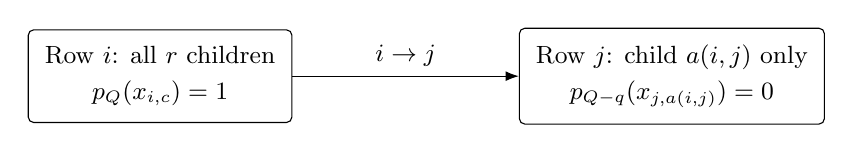
\begin{tikzpicture}[>=Latex, every node/.style={font=\small},
  condition/.style={draw,rounded corners=2pt,inner sep=6pt,align=center}]
 \node[condition] (target) at (0,0)
   {Row \(i\): all \(r\) children\\[2pt] \(p_Q(x_{i,c})=1\)};
 \node[condition] (gate) at (6.5,0)
   {Row \(j\): child \(a(i,j)\) only\\[2pt] \(p_{Q-q}(x_{j,a(i,j)})=0\)};
 \draw[->] (target) -- node[above]{\(i\to j\)} (gate);
\end{tikzpicture}
\caption{Clause $i$ at index $q$: $r$ targets in row $i$, and one gate in each
of the $M^2$ rows $j$ with $i\to j$.}
\label{fig:clause}
\end{figure}

\subsection{Sensitivity profiles and the initial bounds}
For \(b\in\{0,1\}\) define
\[
 S_{\ell,b}=\max_{\substack{1\le q\le H_\ell,\ x\in\{0,1\}^{N_\ell}\\
                           P_{\ell,q}(x)=b}}
 \bigl|\{e\in[N_\ell]:P_{\ell,q}(x^e)=1-b\}\bigr|,
\]
\[
 J_{\ell,b}=\max_{\substack{1\le q<q'\le H_\ell,\ x\in\{0,1\}^{N_\ell}\\
                         P_{\ell,q}(x)=P_{\ell,q'}(x)=b}}
 \bigl|\{e\in[N_\ell]:P_{\ell,q}(x^e)=P_{\ell,q'}(x^e)=1-b\}\bigr|.
\]
So $S_{\ell,b}$ bounds the number of coordinates whose flip moves one
predicate from $b$ to $1-b$, and $J_{\ell,b}$ the number whose flip moves two
distinct predicates from $b$ to $1-b$ at once. An empty maximum is zero; in
particular \(J_{d,0}=J_{d,1}=0\), since \(H_d=1\).

\begin{lemma}\label{lem:base}
The initial sensitivity profiles satisfy
\begin{equation}\label{eq:base-profile}
 S_{0,0}\le L,\qquad S_{0,1}\le LM,\qquad
 J_{0,0}=J_{0,1}=0.
\end{equation}
\end{lemma}
\begin{proof}
\emph{$S_{0,0}$.} Fix $q$, put \(R=d+1-q\in\{0,\ldots,d\}\), and let $x$
satisfy $D(x)>R$. Suppose $D(x^e)\le R$, so
$\operatorname{dist}(x^e,z_j)\le R$ for some $j$; then
$\operatorname{dist}(x,z_j)\le R+1\le d+1$. At most one centre lies within
distance \(d+1\) of \(x\), since two would be within \(2d+2<2L\) of each
other. So $j$ does not depend on $e$. Also
$\operatorname{dist}(x,z_j)\ge D(x)\ge R+1$, hence
$\operatorname{dist}(x,z_j)=R+1$, and $e$ must be one of the $R+1$ coordinates
where $x$ and $z_j$ differ. This gives at most \(R+1\le d+1\le L\) flips.

\emph{$S_{0,1}$.} There are only \(LM\) coordinates.

\emph{$J_{0,b}$.} If $x,y$ differ in one coordinate, the triangle inequality
gives \(|D(x)-D(y)|\le1\). Let $q<q'$, with radii $R=d+1-q$ and $R'=d+1-q'$,
so $R\ge R'+1$. If both predicates are $0$ at $x$ and $1$ at $x^e$, then
$D(x)\ge R+1\ge R'+2$ and $D(x^e)\le R'$. If both are $1$ at $x$ and $0$ at
$x^e$, then $D(x)\le R'$ and $D(x^e)\ge R+1\ge R'+2$. Either way $D$ changes
by at least two, which is impossible.
\end{proof}

\subsection{Disjoint blocks at zero}
\begin{lemma}\label{lem:blocks}
At every level \(0\le\ell\le d\), all predicates are zero at the
all-zero input. There are \(Mk^\ell\) pairwise disjoint nonempty blocks
of coordinates, each of size \(Lr^\ell\), such that flipping any one
block at zero makes every predicate at that level equal to one.
\end{lemma}
\begin{proof}
Induction on $\ell$. \emph{Level $0$:}
$\operatorname{dist}(0,z_j)=L$ for all $j$, so \(D(0)=L>d\) and all
predicates vanish at $0$. The $M$ blocks \(E_j\) work, since \(0^{E_j}=z_j\)
has $D=0$.

\emph{Level $\ell\ge1$:} at the all-zero input every child is all-zero, so
$p_Q=0$ on every child by induction; every target, hence every clause, fails,
and all $P_{\ell,q}(0)=0$. Let \(B_1,\ldots,B_{Mk^{\ell-1}}\) be the
level-$(\ell-1)$ blocks. For each row \(i\) and each \(h\), let $B_{i,h}$ be
the union of the copies of \(B_h\) in the \(r\) children of row \(i\). After
flipping $B_{i,h}$ at $0$:
\begin{itemize}[leftmargin=*,itemsep=1pt]
\item each child of row $i$ equals $0^{B_h}$, so $p_Q=1$ there by induction:
 all targets of clause $i$ hold;
\item children in other rows are still all-zero, so every $p_\gamma$ is $0$
 on them: all gates of clause $i$ hold, for every $q$.
\end{itemize}
Thus every \(P_{\ell,q}\) equals one. The $B_{i,h}$ are pairwise disjoint
(different rows use different children; within a row the $B_h$ are disjoint in
each child). There are \(k\cdot Mk^{\ell-1}=Mk^\ell\) of them, each of size
\(r\cdot Lr^{\ell-1}=Lr^\ell\).
\end{proof}

\section{Sensitivity recurrences}
\label{sec:recurrences}

\begin{proposition}\label{prop:recurrences}
For $1\leq \ell\leq d$, write
$S'_b=S_{\ell-1,b}$ and $J'_b=J_{\ell-1,b}$.  Then
\begin{equation}\label{eq:recurrences}
\begin{aligned}
 S_{\ell,1}&\leq M^2S'_0+rS'_1,
 &\qquad J_{\ell,1}&\leq M^2J'_0+rS'_1,\\
 S_{\ell,0}&\leq tS'_0+S'_1+3J'_1,
 &\qquad J_{\ell,0}&\leq tS'_0+3J'_1.
\end{aligned}
\end{equation}
\end{proposition}

\emph{Plan.} A flip changes a parent predicate only by breaking or completing
a clause, and by (DC) it does so through exactly one condition on one child.
We count, child by child, the flips that reverse that condition, using
$S'_b$ when one child predicate must change and $J'_b$ when two must change.
Parts A--B treat inputs of value $1$ (one fixed satisfied clause);
Parts C--D treat inputs of value $0$, where the task is to bound the number
of clauses one flip away from being satisfied.

\begin{proof}
Fix $\ell$ and use $H$, $Q$, $p_\gamma$ as in
Section~\ref{sec:construction}. In Parts B and D we write
$\gamma=Q-q$, $\gamma'=Q-q'$ (the source's $g,g'$; renamed because $g$ is a
function in Lemma~\ref{lem:composition}). A ``flip'' always means flipping one
coordinate $e$ of the level-$\ell$ input; $e$ lies in exactly one child. If
$H=1$ the two $J$-inequalities hold trivially (empty maximum), so in Parts B
and D assume $H\ge2$.

\smallskip\noindent\textbf{Three tools.}
By the definitions of $S'_b$ and $J'_b$, for every child $y$ and $b\in\{0,1\}$:
\begin{description}[leftmargin=*,itemsep=1pt]
\item[\textup{(S$'$)}] for each $\gamma\in[Q]$, at most $S'_b$ coordinates of
 $y$ have a flip changing $p_\gamma(y)$ from $b$ to $1-b$;
\item[\textup{(J$'$)}] for each $1\le\gamma'<\gamma\le Q$, at most $J'_b$
 coordinates of $y$ have a flip changing both $p_{\gamma'}(y)$ and
 $p_\gamma(y)$ from $b$ to $1-b$.
\item[\textup{(SF)}] \emph{Single-flip principle.} Let $w,w'$ differ in one
 coordinate $e$, and suppose clause $i$ (at a fixed index) fails at $w$ and
 holds at $w'$. Then exactly one condition of clause $i$ fails at $w$, and it
 sits on the child containing $e$. Reason: some condition fails at $w$, none
 fails at $w'$, and by (DC) only the condition on the child containing $e$ can
 differ between $w$ and $w'$.
\end{description}

\smallskip\noindent\textbf{Part A: $S_{\ell,1}\le M^2S'_0+rS'_1$.}
Fix $q$ and $x$ with $P_{\ell,q}(x)=1$, and fix one clause $i$ that holds at
$x$. If $P_{\ell,q}(x^e)=0$, clause $i$ fails at $x^e$, so by (SF) (with
$w=x^e$, $w'=x$) the coordinate $e$ lies in one of the $r+M^2$ children of
clause $i$ and reverses the condition there. On a target child this means
$p_Q$ goes $1\to0$: at most $S'_1$ choices of $e$ by (S$'$). On a gate child
it means $p_{Q-q}$ goes $0\to1$: at most $S'_0$ choices. Summing over $r$
target and $M^2$ gate children gives the bound.

\smallskip\noindent\textbf{Part B: $J_{\ell,1}\le M^2J'_0+rS'_1$.}
Fix $q<q'$ and $x$ with $P_{\ell,q}(x)=P_{\ell,q'}(x)=1$; then
$1\le\gamma'<\gamma<Q$. Fix a clause $i$ that holds at $x$ at index $q'$; by
(Mon) it also holds at index $q$. Let $e$ satisfy
$P_{\ell,q}(x^e)=P_{\ell,q'}(x^e)=0$. Since $P_{\ell,q}(x^e)=0$, clause $i$
fails at $x^e$ at index $q$. By (SF) at index $q$, $e$ lies in a child $y$ of
clause $i$ whose index-$q$ condition holds before and fails after the flip.
\begin{itemize}[leftmargin=*,itemsep=1pt]
\item \emph{$y$ is a target child.} Then $p_Q(y)$ goes $1\to0$: at most
 $S'_1$ such $e$ per target child, $rS'_1$ in all.
\item \emph{$y$ is a gate child.} Before the flip, $p_{\gamma'}(y)=0$ (the
 index-$q'$ gate holds) and $p_\gamma(y)=0$ (the index-$q$ gate holds). After
 the flip $p_\gamma(y)=1$ (the index-$q$ gate fails), hence
 $p_{\gamma'}(y)=1$ by (N). Both $p_{\gamma'}$ and $p_\gamma$ go $0\to1$, so
 by (J$'$) there are at most $J'_0$ such $e$ per gate child, $M^2J'_0$ in all.
\end{itemize}

\smallskip\noindent\textbf{Part C: $S_{\ell,0}\le tS'_0+S'_1+3J'_1$.}
Fix $q$ and $x$ with $P_{\ell,q}(x)=0$; every clause fails at $x$. Put
$\gamma=Q-q<Q$.

\emph{C1 (candidate lists).} Let $\mathcal T$ be the set of $i\in[k]$ whose
clause fails exactly one target and no gate at $x$, and $\mathcal G$ the set
of $i$ whose clause fails exactly one gate and no target. Both depend only on
$x$ and $q$. If $P_{\ell,q}(x^e)=1$, some clause $i$ holds at $x^e$; by (SF),
$i\in\mathcal T\cup\mathcal G$, and $e$ lies in the child of the unique failed
condition of clause $i$ and makes that condition true. For
$i\in\mathcal T\cup\mathcal G$ let $\rho_i$ be the number of coordinates of
that child whose flip makes that condition true. By the union bound, the
number of $e$ with $P_{\ell,q}(x^e)=1$ is at most
$\sum_{i\in\mathcal T}\rho_i+\sum_{i\in\mathcal G}\rho_i$.

\emph{C2 ($|\mathcal T|\le t-1$ and $\rho_j\le S'_0$ for
$j\in\mathcal T$).} For $j\in\mathcal T$ let $m_j\in[r]$ be the position of
its failed target: $p_Q(x_{j,m_j})=0$ and $p_Q(x_{j,c})=1$ for $c\ne m_j$.
Let $i,j\in\mathcal T$ with $i\to j$. Clause $i$ fails no gate, so
$p_\gamma(x_{j,a(i,j)})=0$, and by (N) (as $\gamma<Q$)
$p_Q(x_{j,a(i,j)})=0$. The only position of row $j$ where $p_Q$ vanishes is
$m_j$, so $a(i,j)=m_j$. If $|\mathcal T|\ge t$, any $t$-subset
$I\subseteq\mathcal T$ with the numbers $(m_j)_{j\in I}$ would contradict
Lemma~\ref{lem:labelling}. Hence $|\mathcal T|\le t-1$. Repairing clause
$j\in\mathcal T$ means changing $p_Q(x_{j,m_j})$ from $0$ to $1$, so
$\rho_j\le S'_0$ by (S$'$), and
$\sum_{j\in\mathcal T}\rho_j\le tS'_0$.

\emph{C3 ($|\mathcal G|\le3$).} For $j\in\mathcal G$ all targets hold:
\[
 p_Q(x_{j,c})=1\ \text{ and hence, by (N), }\ p_\gamma(x_{j,c})=1
 \qquad\text{for all }c\in[r].\tag{$\star$}
\]
Let $i,j\in\mathcal G$ with $i\to j$. By $(\star)$,
$p_\gamma(x_{j,a(i,j)})=1$, so the gate of clause $i$ on edge $i\to j$ fails.
Clause $i$ has exactly one failed gate, so $i$ has at most one out-neighbour
in $\mathcal G$. Write $w=|\mathcal G|$ (the source's $m$). The tournament
restricted to $\mathcal G$ has $w(w-1)/2$ edges and at most $w$ (one per
tail), so $w(w-1)/2\le w$, i.e.\ $w\le3$. Moreover at most one vertex of
$\mathcal G$ has no out-neighbour in $\mathcal G$, since of any two vertices
one points to the other.

\emph{C4 (counting $\mathcal G$).} Let $i\in\mathcal G$.
\begin{itemize}[leftmargin=*,itemsep=1pt]
\item[(a)] \emph{$i$ has an out-neighbour $j\in\mathcal G$.} By C3 its unique
 failed gate sits on $y=x_{j,a(i,j)}$, where $p_\gamma(y)=p_Q(y)=1$ by
 $(\star)$. Repairing the gate makes $p_\gamma(y)=0$, and then $p_Q(y)=0$ by
 (N). So two distinct child predicates ($\gamma<Q$) go $1\to0$, and
 $\rho_i\le J'_1$ by (J$'$). (That this flip breaks a target of clause $j$ is
 irrelevant: we only bound $\rho_i$ from above.)
\item[(b)] \emph{$i$ has no out-neighbour in $\mathcal G$} (at most one such
 $i$). Repairing its failed gate changes $p_\gamma$ from $1$ to $0$ on one
 child, so $\rho_i\le S'_1$ by (S$'$).
\end{itemize}
Since $|\mathcal G|\le3$, $\sum_{i\in\mathcal G}\rho_i\le S'_1+3J'_1$.
With C1 and C2 this proves Part C.

\smallskip\noindent\textbf{Part D: $J_{\ell,0}\le tS'_0+3J'_1$.}
Fix $q<q'$ and $x$ with $P_{\ell,q}(x)=P_{\ell,q'}(x)=0$; again
$1\le\gamma'<\gamma<Q$. Let $\mathcal T,\mathcal G$ be the lists of Part C for
$x$ and the \emph{smaller} index $q$; so $|\mathcal T|\le t-1$ and
$|\mathcal G|\le3$. Let $e$ satisfy
$P_{\ell,q}(x^e)=P_{\ell,q'}(x^e)=1$, and choose a clause $i$ that holds at
$x^e$ at index $q'$ (the choice may depend on $e$; the lists do not). By (Mon)
clause $i$ holds at $x^e$ at index $q$, and it fails at $x$ at index $q$. By
(SF) at index $q$, $i\in\mathcal T\cup\mathcal G$ and $e$ lies in the child
$y$ of its unique index-$q$ failed condition.
\begin{itemize}[leftmargin=*,itemsep=1pt]
\item \emph{$i\in\mathcal T$.} Then $e$ changes $p_Q(x_{i,m_i})$ from $0$ to
 $1$; as in C2 there are at most $S'_0$ such $e$ per $i$, at most $tS'_0$ in
 all.
\item \emph{$i\in\mathcal G$.} Then $y$ is the child of the failed index-$q$
 gate, so $p_\gamma(y)=1$ before the flip, and $p_{\gamma'}(y)=1$ by (N).
 After the flip clause $i$ holds at index $q'$, so its gate on $y$ gives
 $p_{\gamma'}(y)=0$, and then $p_\gamma(y)=0$ by (N). Both $p_{\gamma'}$ and
 $p_\gamma$ go $1\to0$, so by (J$'$) there are at most $J'_1$ such $e$ per
 $i\in\mathcal G$, at most $3J'_1$ in all.
\end{itemize}
The second case never used $(\star)$: the second changing predicate is
$p_{\gamma'}$, supplied by the index $q'$, instead of $p_Q$. So it covers the
vertex of case C4(b) too, and no $S'_1$ term appears. (The witness $i$ also
has exactly one failed condition at index $q'$ at $x$, by (SF) at index $q'$;
members of $\mathcal T\cup\mathcal G$ with more failures at index $q'$ are
never witnesses and are merely over-counted.)

Every bound holds for all admissible $q$ (or $q<q'$) and $x$; taking maxima
gives~\eqref{eq:recurrences}.
\end{proof}

\section{Quantitative bounds and separation}
\label{sec:separation}

\begin{lemma}
\label{lem:quantitative-profiles}
Suppose that $d\geq 1$ and $M\geq 9^{d+1}$.
For every $0\leq\ell\leq d$ and $b\in\{0,1\}$, the predicates of the
construction satisfy
\[
  S_{\ell,b}\leq 2L M^{\ell+b}.
\]
\end{lemma}

\emph{Plan.} The dominant terms $M^2S'_0$ and $S'_1$ in
\eqref{eq:recurrences} suggest dividing $S_{\ell,b}$ and $J_{\ell,b}$ by
$M^{\ell+b}$. This gives a two-term linear recurrence in which the joint
quantity is fed only through a small coefficient $\epsilon$ but can triple at
each level. The hypothesis $M\ge9^{d+1}$ makes $\epsilon\le2/3^{d+1}$, which
beats $3^d$. Used in the proof of Theorem~\ref{thm:main}.

\begin{proof}
Define
\[
 u_\ell=\max_{b\in\{0,1\}}\frac{S_{\ell,b}}{M^{\ell+b}},
 \qquad
 v_\ell=\max_{b\in\{0,1\}}\frac{J_{\ell,b}}{M^{\ell+b}},
 \qquad
 \epsilon=\frac{\max(r,t)}{M}.
\]

\emph{Step 1 (base).} By~\eqref{eq:base-profile}, $S_{0,0}/M^0\le L$ and
$S_{0,1}/M\le L$, so $u_0\leq L$; and $v_0=0$.

\emph{Step 2 (normalised recurrences).} Let $1\le\ell\le d$. By definition
$S'_b\le M^{\ell-1+b}u_{\ell-1}$ and $J'_b\le M^{\ell-1+b}v_{\ell-1}$.
Dividing~\eqref{eq:recurrences} by $M^{\ell+1}$ (case $b=1$) or $M^\ell$ (case
$b=0$):
\begin{align*}
 \frac{S_{\ell,1}}{M^{\ell+1}}
   &\le\frac{S'_0}{M^{\ell-1}}+\frac rM\cdot\frac{S'_1}{M^{\ell}}
   \le\Bigl(1+\frac rM\Bigr)u_{\ell-1},\\
 \frac{S_{\ell,0}}{M^\ell}
   &\le\frac tM\cdot\frac{S'_0}{M^{\ell-1}}+\frac{S'_1}{M^\ell}+\frac{3J'_1}{M^\ell}
   \le\Bigl(1+\frac tM\Bigr)u_{\ell-1}+3v_{\ell-1},\\
 \frac{J_{\ell,1}}{M^{\ell+1}}
   &\le\frac{J'_0}{M^{\ell-1}}+\frac rM\cdot\frac{S'_1}{M^{\ell}}
   \le\frac rM u_{\ell-1}+v_{\ell-1},\\
 \frac{J_{\ell,0}}{M^\ell}
   &\le\frac tM\cdot\frac{S'_0}{M^{\ell-1}}+\frac{3J'_1}{M^\ell}
   \le\frac tM u_{\ell-1}+3v_{\ell-1}.
\end{align*}
Taking maxima over $b$, and using $v_{\ell-1}\le3v_{\ell-1}$,
\begin{equation}
\label{eq:normalized-recurrences}
  u_\ell\leq (1+\epsilon)u_{\ell-1}+3v_{\ell-1},\qquad
  v_\ell\leq \epsilon u_{\ell-1}+3v_{\ell-1}.
\end{equation}

\emph{Step 3 (size of $\epsilon$).} Since $M\ge9^{d+1}\geq81$, we have
$r=\lceil\sqrt M\rceil\leq\sqrt M+1\le2\sqrt M$ and
$t=16\leq2\sqrt M$. With $\sqrt M\ge3^{d+1}$,
\begin{equation}
\label{eq:epsilon-choice}
 \epsilon\leq\frac{2}{\sqrt M}\leq\frac{2}{3^{d+1}}.
\end{equation}

\emph{Step 4 (comparison sequences).} Let $U_0=L$, $V_0=0$ and
\[
 U_\ell=(1+\epsilon)U_{\ell-1}+3V_{\ell-1},
 \qquad
 V_\ell=\epsilon U_{\ell-1}+3V_{\ell-1}.
\]
All coefficients are nonnegative, so Step~1
and~\eqref{eq:normalized-recurrences} give $u_\ell\leq U_\ell$,
$v_\ell\leq V_\ell$ by induction on $\ell$.

\emph{Step 5.} We show by induction that for $0\leq\ell\leq d$,
\begin{equation}
\label{eq:comparison-bounds}
 U_\ell\leq2L,
 \qquad
 V_\ell\leq\epsilon L(3^\ell-1).
\end{equation}
Both hold at $\ell=0$. Assume them for all indices below some
$1\leq\ell\leq d$. First,
\[
 V_\ell=\epsilon U_{\ell-1}+3V_{\ell-1}
 \leq 2\epsilon L+3\epsilon L(3^{\ell-1}-1)
 =\epsilon L(3^\ell-1).
\]
Next, $U_{j+1}-U_j=\epsilon U_j+3V_j$; summing over $j<\ell$ and using
$\sum_{j=0}^{\ell-1}(3^j-1)=\tfrac12(3^\ell-1)-\ell$,
\begin{align*}
 U_\ell
 &=L+\sum_{j=0}^{\ell-1}(\epsilon U_j+3V_j)
 \leq L+2\epsilon L\ell+3\epsilon L\Bigl[\frac{3^\ell-1}{2}-\ell\Bigr]
 =L+\epsilon L\Bigl[\frac32(3^\ell-1)-\ell\Bigr].
\end{align*}
By~\eqref{eq:epsilon-choice} and $\ell\le d$,
\[
 \epsilon\Bigl[\frac32(3^\ell-1)-\ell\Bigr]
 \leq\frac{2}{3^{d+1}}\cdot\frac{3^{\ell+1}-3-2\ell}{2}
 =\frac{3^{\ell+1}-3-2\ell}{3^{d+1}}<1,
\]
so $U_\ell<2L$. This completes the induction. Hence
$S_{\ell,b}\le M^{\ell+b}u_\ell\le M^{\ell+b}U_\ell\leq2LM^{\ell+b}$.
\end{proof}

\begin{proof}[Proof of Theorem~\ref{thm:main}]
Fix an integer $d\geq1$ and an integer $M\geq9^{d+1}$ (so $M\ge3$), and a
labelling from Lemma~\ref{lem:labelling}. Following Ambainis and Sun
\cite[Section~4, Lemma~1]{AmbainisSun2011}, let $f$ be the OR of $M$ copies of
$P_{d,1}$ on disjoint sets of variables. Each copy has $LM(kr)^d$ variables,
so $f$ is a total Boolean function on
\begin{equation}
\label{eq:final-dimension}
 n=LM^2(kr)^d
\end{equation}
bits.

\emph{Step 1 ($f(0)=0$, and block sensitivity).} By Lemma~\ref{lem:blocks}
every copy is $0$ at its zero input, so $f(0)=0$. Each copy has $Mk^d$
pairwise disjoint blocks whose flip at zero makes that copy, hence $f$, equal
to $1$. Over the $M$ disjoint copies this gives $M^2k^d$ pairwise disjoint
sensitive blocks of $f$ at $0$:
\begin{equation}
\label{eq:final-block-sensitivity}
 \bs(f,0)\geq M^2k^d.
\end{equation}
In particular $f$ is nonconstant, so $s(f)>0$.

\emph{Step 2 (sensitivity).} Let $f(x)=0$. Then every copy is $0$, and a flip
changes $f$ only if it turns its own copy to $1$; there are at most $S_{d,0}$
such flips per copy, so $s(f,x)\le MS_{d,0}$. Let $f(x)=1$. If at least two
copies accept, no single flip makes $f$ zero. If exactly one accepts, a
sensitive flip must lie in that copy and turn it to $0$, so
$s(f,x)\le S_{d,1}$. By Lemma~\ref{lem:quantitative-profiles},
\begin{equation}
\label{eq:final-sensitivity}
 s(f)\leq\max\{M S_{d,0},S_{d,1}\}
       \leq\max\{M\cdot2LM^d,\,2LM^{d+1}\}=2L M^{d+1}.
\end{equation}

\emph{Step 3 (ratio).} By~\eqref{eq:final-sensitivity},
\eqref{eq:final-block-sensitivity}, and $k/M^2>2$,
\begin{equation}
\label{eq:ratio-separation}
 \frac{\bs(f)}{s(f)^2}
 \geq\frac{\bs(f,0)}{s(f)^2}
 \geq\frac{M^2k^d}{4L^2M^{2d+2}}
 =\frac{(k/M^2)^d}{4L^2}
 \geq\frac{2^d}{4(d+2)^2}.
\end{equation}
This proves the second statement. The right-hand side tends to infinity with
$d$. Given $C>0$, choose $d$ with $2^d/(4(d+2)^2)>C$, then $M$, the labelling
and $f$ as above; since $s(f)>0$, $\bs(f)>C s(f)^2$.
\end{proof}

\subsection{A fixed exponent by composition}

Composing the $d=9$ function with itself gives a power separation, by the
composition principle studied by Tal~\cite{Tal2013}. We prove the two facts
needed. In the next lemma the source's dimensions $a,b$, block counts $p,q$
and blocks $C_i,D_j$ are renamed $n_1,n_2$, $p_1,p_2$, $X_i,Y_j$ to avoid
clashes with earlier notation.

\begin{lemma}
\label{lem:composition}
Let $f:\{0,1\}^{n_1}\to\{0,1\}$ and
$g:\{0,1\}^{n_2}\to\{0,1\}$ be total Boolean functions.
Their disjoint composition is the function on $n_1n_2$ bits defined by
\[
 (f\circ g)(x_1,\ldots,x_{n_1})
   =f\bigl(g(x_1),\ldots,g(x_{n_1})\bigr),
 \qquad x_i\in\{0,1\}^{n_2}.
\]
Then
\[
 s(f\circ g)\leq s(f)s(g).
\]
If $g(0)=0$, then $(f\circ g)(0)=f(0)$ and
\[
 \bs(f\circ g,0)\geq\bs(f,0)\bs(g,0).
\]
More explicitly, any disjoint families of $p_1$ and $p_2$ blocks sensitive at
zero for $f$ and $g$, respectively, yield a disjoint family of $p_1p_2$ blocks
sensitive at zero for $f\circ g$.
\end{lemma}

\begin{proof}
\emph{Sensitivity.} For $x=(x_1,\ldots,x_{n_1})$ put
$y=(g(x_1),\ldots,g(x_{n_1}))$. Flipping a coordinate inside $x_i$ leaves $y$
unchanged unless it changes $g(x_i)$, in which case $y$ becomes $y^{\{i\}}$.
So the flip changes $f\circ g$ exactly when it is sensitive for $g$ at $x_i$
and $f(y^{\{i\}})\ne f(y)$. Thus
\[
 s(f\circ g,x)
   =\sum_{i:\,f(y^{\{i\}})\ne f(y)}s(g,x_i)
   \leq s(f,y)s(g)
   \leq s(f)s(g).
\]

\emph{Blocks.} Let $g(0)=0$; then $(f\circ g)(0)=f(0,\ldots,0)=f(0)$. Let
$X_1,\ldots,X_{p_1}\subseteq[n_1]$ and $Y_1,\ldots,Y_{p_2}\subseteq[n_2]$ be
pairwise disjoint sensitive blocks at zero for $f$ and $g$ respectively.
Identify the coordinates of $f\circ g$ with $[n_1]\times[n_2]$. The sets
$X_i\times Y_j$ are nonempty and pairwise disjoint. Flipping $X_i\times Y_j$
at zero turns each child indexed by $X_i$ into $0^{Y_j}$, where $g=1$ (as
$g(0)=0$ and $Y_j$ is sensitive), and leaves the other children at $0$, where
$g=0$. The outer input becomes $0^{X_i}$, the indicator string of $X_i$, and
$f(0^{X_i})\ne f(0)$ because $X_i$ is sensitive for $f$ at zero. So each
$X_i\times Y_j$ is sensitive for $f\circ g$ at zero. Taking maximum families
gives the inequality (trivial if either maximum is zero).
\end{proof}

\begin{corollary}
\label{cor:power-separation}
There exist a real number $\alpha>2$ and nonconstant total Boolean
functions $F_m$, for integers $m\geq1$, such that
\[
 \bs(F_m,0)\geq s(F_m)^\alpha
 \qquad\text{for every }m,
 \qquad
 \bs(F_m,0)\longrightarrow\infty.
\]
\end{corollary}

\begin{proof}
Fix $d=9$ (so $L=11$), an integer $M\geq9^{10}$, and an admissible
labelling; let $f$ be the function from the proof of
Theorem~\ref{thm:main}. Put
\[
 A=22M^{10},\qquad B=M^2k^9.
\]
By~\eqref{eq:final-sensitivity} and~\eqref{eq:final-block-sensitivity},
$s(f)\leq A$ and $\bs(f,0)\geq B$; also $f(0)=0$. Moreover
\[
 \frac{B}{A^2}
   =\frac{M^2k^9}{484M^{20}}
   =\frac{(k/M^2)^9}{484}
   \geq\frac{2^9}{484}
   =\frac{128}{121}>1.
\]
So $A>1$, $B>A^2$, and $\alpha=\log B/\log A>2$. This $\alpha$ depends on the
chosen $M$; it is fixed once $M$ is.

Set $F_1=f$ and $F_{m+1}=f\circ F_m$. We show by induction that $F_m$ is a
total function on $n^m$ bits ($n$ as in~\eqref{eq:final-dimension}) with
\[
 F_m(0)=0,\qquad s(F_m)\leq A^m,\qquad \bs(F_m,0)\geq B^m.
\]
For $m=1$ this was just shown. Given the claim for $m$,
Lemma~\ref{lem:composition} with inner function $F_m$ (allowed since
$F_m(0)=0$) gives $F_{m+1}(0)=f(0)=0$,
$s(F_{m+1})\le s(f)s(F_m)\le A^{m+1}$ and
$\bs(F_{m+1},0)\ge\bs(f,0)\bs(F_m,0)\ge B^{m+1}$.

Since $\bs(F_m,0)\ge B^m\ge1$, $F_m$ has a sensitive block and is
nonconstant, and $\bs(F_m,0)\to\infty$ because $B>1$. Since $A^\alpha=B$,
\[
 s(F_m)^\alpha\leq A^{m\alpha}=B^m\leq\bs(F_m,0).
\]
The same estimates give
\[
 \frac{\bs(F_m)}{s(F_m)^2}
 \geq\left(\frac{B}{A^2}\right)^m
 \geq\left(\frac{128}{121}\right)^m.\qedhere
\]
\end{proof}

\section{Verification checklist}

No step of the source was left unverified in this rewrite. A sceptical reader
should check these load-bearing points first.

\begin{enumerate}[leftmargin=*,itemsep=2pt]
\item \textbf{(DC) and (SF).} Each clause uses each child at most once, so one
 flip changes at most one of its conditions
 (Section~\ref{sec:construction}; ``Three tools'' in the proof of
 Proposition~\ref{prop:recurrences}). All of Parts A--D rest on this.
\item \textbf{Directions of nesting.} $p_\gamma=0\Rightarrow p_Q=0$ in C2;
 $p_Q=1\Rightarrow p_\gamma=1$ in $(\star)$; and in Parts B and D the pair
 $\gamma'<\gamma$ consists of two \emph{distinct} valid indices
 ($1\le\gamma'<\gamma<Q$), as (J$'$) requires.
\item \textbf{Step C2.} The deduction $a(i,j)=m_j$ for every edge inside
 $\mathcal T$ matches exactly the pattern forbidden by
 Lemma~\ref{lem:labelling}; the arithmetic of that lemma is
 $\binom{16}{2}=120$ and $k^{16}r^{-104}\le3^{16}M^{-20}<1$.
\item \textbf{Steps C3--C4.} Out-degree at most one inside $\mathcal G$ gives
 $|\mathcal G|\le3$ with at most one sink; non-sinks cost $J'_1$ (two
 predicates change), the sink costs $S'_1$.
\item \textbf{Part D.} Every witness in $\mathcal G$ costs $J'_1$, with
 $p_{\gamma'}$ as second predicate, so $J_{\ell,0}$ has no $S'_1$ term. This
 absence is what keeps $v_\ell$ small in
 Lemma~\ref{lem:quantitative-profiles}.
\item \textbf{Normalisation.} The exponents in Step~2 of
 Lemma~\ref{lem:quantitative-profiles} (divide by $M^{\ell+b}$), and the final
 inequality $(3^{\ell+1}-3-2\ell)/3^{d+1}<1$, which uses $M\ge9^{d+1}$ and
 $\ell\le d$.
\item \textbf{Lemma~\ref{lem:base}.} Uniqueness of the nearby centre
 ($2d+2<2L$) and the gap of two between distinct radii.
\item \textbf{Final count.} $s(f)\le\max\{MS_{d,0},S_{d,1}\}$ for the OR,
 $\bs(f,0)\ge M^2k^d$, and $k/M^2>2$ (proof of Theorem~\ref{thm:main});
 $B/A^2\ge128/121$ and the use of $F_m(0)=0$ in
 Corollary~\ref{cor:power-separation}.
\end{enumerate}

\bibliographystyle{alpha}
\bibliography{references}
\end{document}
